\documentclass{book}
\usepackage{ctex}
\usepackage{enumerate}
\usepackage{enumitem}   % [inline] option for inline enumerate, following https://tex.stackexchange.com/a/146311
\usepackage[colorlinks]{hyperref}
\usepackage{bookmark}
\usepackage[left=3cm,right=3cm]{geometry}
\usepackage{multicol}
\usepackage[official]{eurosym}
\usepackage{booktabs}
\usepackage{xcolor}
\usepackage{siunitx}
\usepackage{graphicx}
\usepackage{appendix}

\graphicspath{{Images/}}

% Define my "abstract" title, following https://en.wikibooks.org/wiki/LaTeX/Document_Structure#Abstract
\renewcommand{\abstractname}{声明}

\title{Road to TUM\\for UCASer in Summer, 2019}
\author{UCASer 16}
\date{\today}

\begin{document}
\maketitle

% \begin{center}
请务必确认,所填表格为从官方下载的最新版本(如果有)。本文档中的链接为截至 2018 年 12 月下旬的版本,不保证为当前最新版本。

当前进度:关于递签(见 \ref{sec:visa} 节,特别是签证所需材料 \ref{sec:visa-material} 一节),及 1 月 17 日递签资料图表(见 \ref{ap:visa-figures} 节)。

寒假中计划补充“一些建议”一节;添加 ``FAQ'' 一节,后者内容上为其余各节的精简版,但比 ``To-Do List'' 完整。

希望大家随时在 QQ 群里指出有误或写得不清楚的地方。有任何其他建议也可随时在 QQ 群里提出。
% \end{center}

% \vfill

% \abstract{
本文所参考内容将尽可能注明出处。%,且本文骨干内容主要基于:
% \begin{enumerate}          % inline enumerate with *, given [inline] option in package enumitem
%   \item 16级 QQ 群文件 “\href{https://docs.qq.com/doc/DSHd2dlFVZXpodEpq}{TUM 流程}”,
%   \item ZDL 老师邮件的附件,
%   \item TUM Dalma 邮件及其附件。
% \end{enumerate}
文中出现人名的地方,全部(除了附录中联系人姓名。但目前没有逐一检查确认)以姓名的拼音首字母(大写)出现。
% }

文档中各节间安排顺序与实际操作顺序无直接关系。
\vfill

这份文档,既为了方便此次访学,也是希望能够为往后的 TUM 交流生铺一条路。

这份文档由 \LaTeX 写作编译成 pdf. 目前放在 \href{https://www.overlear.com}{overleaf.com} (项目名为 \href{https://www.overleaf.com/2269426218fxwmgyxjywnn}{Road-to-TUM}) 以及 \href{https://github.com}{github.com} (项目名为 \href{https://github.com/Memcys/Road-to-TUM.git}{Road-to-TUM}, 同时有利用 Pandoc 不定期从 .tex 转换为 .docx 的 Word 文档)上。目前 overleaf 网络访问不畅通,故新添了 github 项目。

主要内容的增补将同时在文件“\href{https://docs.qq.com/doc/DSHd2dlFVZXpodEpq}{TUM 流程}”中进行(目前PZY同学贡献了多数内容)。现在这两份文件的分别比较大。希望有兴趣的同学可以参与这个文档编写项目。

目前文档正在增添和修补中。文中“做什么”“建议做什么”“为什么这么做”等杂糅。有些地方指出 见附件 等,是直接粘贴的原句。但附件没有上传。此外,videx, 递签等部分细节仍待补充。各节内容都需补充。中英交替,语言表述不够准确、精炼等情况,暂不处理。

\newpage

\chapter{To-Do List}
(使用合适的 pdf 阅读器,可以点选/取消可选框。)
\begin{Form}
\small
% Following https://tex.stackexchange.com/a/310574
  \begin{enumerate}[label = {\CheckBox[width=.1in,height=.1in,name=process\theenumi]{}}]
  \item 德国保险
    \begin{multicols}{2}
    \begin{enumerate}[label = {\CheckBox[width=.1in,height=.1in,name=subprocess\theenumii]{}} \arabic*.]
      \item (AOK)申请表
      \item certificate for enrollment
      \item email \href{mailto:alagha@zv.tum.de}{alagha@zv.tum.de}
    \end{enumerate}  
    \end{multicols}
  \item 签证申请
  % \begin{multicols}{3}
  \begin{enumerate}[label = {\CheckBox[width=.1in,height=.1in,name=subprocess\theenumii]{}}]
    \item videx form
    \item APS 材料
      \begin{multicols}{2}
      \begin{enumerate}[label = {\CheckBox[width=.1in,height=.1in,name=subsubprocess\theenumiii]{}} \arabic*.]
        \item APS 注册
        \item 身份证,护照复印件
        \item 在学证明原件
        \item 成绩单原件
        \item 录取花名册相关页原件
        \item 中德负责人联系方式
        \item 汇款单收据的复印件
      \end{enumerate}
      \end{multicols}
    \item 递签材料原件(除了护照,似乎没有强制要求顺序)
      \begin{multicols}{2}
        \begin{enumerate}[label = {\CheckBox[width=.1in,height=.1in,name=subsubprocess\theenumiii]{}} \arabic*.]
          \item 护照(首页用曲别针夹一张白底二寸照片)
          \item 录取证明
          \item 资金证明
          \item 在读证明
          \item 保险证明
          \item 审核证书
          \item VIDEX 二维码
          \item EMS 快递单(见 \ref{visa-EMS})
        \end{enumerate}
      \end{multicols}
    \item 递签材料复印件(2 套。放置顺序有上到下)
      \begin{multicols}{2}
      \begin{enumerate}[label = {\CheckBox[width=.1in,height=.1in,name=subsubprocess\theenumiii]{}} \arabic*.]
      % \item 1 份 videx 表格最后页(英文第 7 页)
      \item 德文签证申请表(首页粘贴白底二寸护照照片,地址栏为现居地址,末页中文签名)
      \item 签证申请补充声明(文件名为“联系方式及代办人的附加证明”。中文签名)
      \item 护照首页复印件
      \item TUM 通知书(并通知信)
      \item 存款证明复印件
      \item 语言水平证明复印件
      \item 在学证明(并附\textbf{德文翻译})
      \item \textbf{德文}个人简历
      \item \textbf{德文}留学动机说明
      \item 审核证书复印件
      \item 入境后医疗保险证明(见 \ref{ensurance-Versicherungsbescheinigung} )复印件
      \item 保险声明%(见 \ref{inline-ensurance-acknowledgement}。放置顺序未知)
      {\color{gray}\\
      以下内容不是图 \ref{fig:order-1}, \ref{fig:order-2} 所要求的递签材料。但现金请务必带上。
      \item 现金(不少于 33 元人民币。见 \ref{inline-money} 及 \ref{print-fee})
      \item 预约递签的回复邮件打印版(出处待补充。递签时似乎未提交该材料)
      }
      \end{enumerate}
      \end{multicols}
    \item 德意志银行开户
      \begin{multicols}{2}
      \begin{enumerate}[label = {\CheckBox[width=.1in,height=.1in,name=subsubprocess\theenumiii]{}} \arabic*.]
        \item 开户表格(2 份,单面)
        \item 资金来源证明(中英文)
        \item 护照、身份证原件 + 1 份复印件
        \item TUM 通知书 A4 单面
        \item 登记卡(手写)
        \item 人民币 850 元(半年期)/ 1200 元(一年期)%(二者均可。注意,转账时仍可能按比例扣除手续费。实际为汇款)
      \end{enumerate}
      \end{multicols}
    \item APS 预约递签
    \item APS 递签
    \item 领取护照 (EMS?)
    % \item APS 的审核证明/审核证书/传真
  \end{enumerate}
  % \end{multicols}
  \item 德国居留许可申请
  \item 住宿
  \item 航班
  \item Registration for TUM
  \begin{multicols}{2}
  \begin{enumerate}[label = {\CheckBox[width=.1in,height=.1in,name=subprocess\theenumii]{}}]
    \item \euro{129,40}
    \item health insurance
    \item up-load a photo in TUMonline (and change password)
  \end{enumerate}
  \end{multicols}
  \end{enumerate}
\end{Form}

% \newpage
\tableofcontents
\listoftables
\listoffigures
% \newpage

\chapter{德国保险}
到德国留学的学生,每人均需购买一份医疗保险才能成功申请签证。%有关医疗保险的细节如下:
\begin{itemize}
\item 可选择购买保险的公司及相应价格如下表:%! figure or table needed here
TUM 给的建议是选择 AOK 公司。
\item 保险购买步骤
\begin{enumerate}
\item 将本人姓名、出生日期、国籍、性别 (Name,Date of birth,Home country,Sex) 等基本信息写邮件至 \sloppy \href{mailto:muenchen.student@service.by.aok.de}{muenchen.student@service.by.aok.de};% Insert email address. Following https://tex.stackexchange.com/a/276.
\item 等对方回邮件填写申请表并签名,TUM官网有 AOK 申请表(见附件2),仅供参考,请以上述邮箱发过来的表格为准;
\item 申请表填好后,打印 application 并填写,扫描后 ``together with a copy of your passport and admission letter of the university'' 发邮件回去。%将扫描件发至给大家发申请表的邮箱地址,
通常一天之后大家就能收到入学所需的保险证明(certificate for enrollment);
% \item 拿到保险公司的保险证明(一个名为 Versicherungsbescheinigung 的文件),将保险证明通过电子邮件发给TUM的负责人Dalma Alagha(\href{mailto:alagha@zv.tum.de}{alagha@zv.tum.de}) (by mentioning your name and your TUM regisration number ``Matrikelnummer''. 见 )
\end{enumerate}
\item TUM保险购买的详细英文指南,以及关于保险的各项细节见附件3;
\end{itemize}

\chapter{签证申请}
\section{签证类型}
申请德国长期签证---留学签证。 
按照短期交换团组的程序申请签证,团组号由访学办老师联系德国大使馆申请,访学办老师取得团组号之后会将团组号告诉所有学生。
短期交换程序的基本流程及要求见附件4

\section{申请流程}
\begin{enumerate}
\item 登录 \url{http://videx.diplo.de/} 填写申请表并下载打印;
\item \sloppy 在德国驻华大使馆留德人员审核部 APS (\url{www.aps.org.cn/zh/}) 注册帐号。\url{https://www.aps.org.cn/zh/verfahren-und-services-deutschland/austauschverfahren}。注册时需要填写 14 位考生号。);
\item 预约递签。网址 \url{https://service2.diplo.de/rktermin/extern/choose_category.do?locationCode=peki&realmId=12&categoryId=156&request_locale=de}. 请以德文界面进入。后续表格中将有 德/英/中 三语。我以英语进入时,表格中多项标题为空白。 
\item 递签,并缴纳申请费(60 欧元,以人民币支付)。
\item 领取护照(6 周以上)。
\end{enumerate}

\section[德意志银行开户]{德意志银行开户}
开户的体验在 \ref{ap:bank} 附录中有补充完善。

本节以下内容参考\href{https://china.db.com/china/docs/Deutsche_Bank-China-Account-Opening-Process-And-Introduction.pdf}{开户流程介绍及登记卡}。

工作时间:(北京分行和上海分行) 周一至周五,上午 9:30 --- 11:30 (公共假期除外)

\begin{table*}[htbp]
\caption{学生业务专线查询(北京分行)}
\label{tb:bank-communication}
\centering
\begin{tabular}{ll}
  垂询电话:(010) 59698181 & 传真:(010) 59695710 \\
  \multicolumn{2}{l}{地址:中国北京市朝阳区建国路81号华贸中心1号写字楼27层(100025)}
\end{tabular}  
\end{table*}

\emph{重要通知}(见德意志银行网页\href{https://china.db.com/china/cn/content/5777.html}{其他信息下载})
\begin{enumerate}
\item 开户表格内容请用电脑在线填写,然后选用A4纸张,单面打印两份(其中一份您自行保留),签字部分由学生本人用黑色墨水笔签写,手工填写的表格无法受理。
\item 开户表格红色标识的区域为必填项,如打印时,页面底部有 ``UNGULTIG'' 字样的提示,表示您还有未完成的部分,请参考填写说明仔细检查。
\item \sloppy 关于允许 Java 脚本运行的提示,请根据您电脑的设置接受或直接填写,需要注意的是,最终提交的表格不能带有 ``UNGULTIG'' 字样。如果本网站提供的表格您始终无法正常打印,可以尝试从我行德国官网提供的表格链接在线填写并打印,网址如下:\\
\url{https://www.deutsche-bank.de/pfb/content/pk-konto-und-karte-international-students.html?pfb_tab=34880-34884}
\item 开户表格中纳税人信息必须填写。要求提供“资金来源证明”,请注意提前准备。
\end{enumerate}
\begin{itemize}
\item 在德意志银行官网上 \url{https://china.db.com/china/cn/content/5777.html} 下载开户表格。填写方法可以按照样表,也可以在以下网站上找到填写攻略:\\
\url{https://www.sohu.com/a/238196417_100189530} (比较全)\\
\url{https://www.sohu.com/a/218431242_507614}
\item 需要准备资金来源证明原件(中英文。办理人不能为学生本人---德国使馆将认定留学生本人无收入。需要冻结资产,欧元形式。冻结时间:最好是冻结到我们去开户的前一天或者当天---\url{http://toutiao.manqian.cn/wz_9HOPNjkAgR.html}。该证明上时间只需持续一天。如 2018 年 12 月 20 日至 2018 年 12 月 21 日---\url{http://toutiao.manqian.cn/wz_16ASBZf2o3.html?tdsourcetag=s_pctim_aiomsg}. );
\item 单面打印两份开户表格,一份自留。 ZJR 建议携带笔记本电脑和 U 盘,因可能需要随时修改;
\item 护照、身份证原件,复印件一份。复印件请以 1:1 比例清晰复印在 A4 纸上(阶梯教室打印店的质量即可);
\item 德国学校提供的大学入学通知书 A4 单面打印;
\item 登记卡。手写。下载链接: \url{https://china.db.com/china/cn/content/5777.html} 中的\href{https://china.db.com/china/docs/Deutsche_Bank-China-Account-Opening-Process-And-Introduction.pdf}{登记卡};
\item 人民币现金 850 元(一年限制题款账户) / 1200 元(半年限制题款账户)。二者均可。注意,转账时仍可能按比例扣除手续费。实际为汇款。去中国银行、工商银行均需当前银行卡,暂不接受现金汇款。
\end{itemize}
% “北京开户是在一楼登记处登记,然后上 27 楼,进去拿号排队,提交开户材料,分行审核通过后,做手续费的汇款”。“手续费包括了国际快递费和分行手续费,共计人民币 850 元(直接汇款即可)”%! link needed here
% (该段文字出处待补充)

\section{留德人员审核部 (APS) 的审核证明(一份原件)}
\begin{enumerate}
  \item 在APS官网填表(选择短期交换项目,团队号见微信群),打印签字,自贴照片(“必须提交 3 张相同的白色背景的近期证件照,照片尺寸为 \SI{45x35}{\mm}. 照片必须为正面免冠照,不能遮挡眼睛。具体要求请参看 \href{https://china.diplo.de/blob/1090226/8b25f160e56c0465aa9b5d5d19f89c4f/pdf-fotomustertafel-data.pdf}{照片示例表}。”---\href{https://china.diplo.de/cn-zh/service/visa-einreise/faq-national-visa/1434978}{长期停留常见问题--9.})
  \item 身份证,护照复印件
  \item 大学在学证明原件(周三下午 13:30--16:30)。\href{https://www.aps.org.cn/wp-content/uploads/260_merkblatt_verfahren_austausch_chn.pdf}{短期交换程序须知}---“大学在读证明内容必须包括:被哪所大学录取,院系名称,所学专业,学号,学历类型,学习起\emph{止}(但老师不允许写该“止”,只允许模板上已有的内容)时间,已读完的学期数(老师勉强允许填写),并由教务处/档案室/学籍管理办公室等校级部门盖章。“
  \item 学士成绩单原件,分学年(本校只提供不分学年的成绩单。周一下午和周三上午,办公室110)。\href{https://www.aps.org.cn/wp-content/uploads/260_merkblatt_verfahren_austausch_chn.pdf}{短期交换程序须知}---“大学成绩单必须包括大学期间所学全部课程的成绩,需要分学期开具,并由教务处/档案室/学籍管理办公室等校级部门盖章。”
  \item 大学录取花名册相关页原件(联系学校招生办开具,先打电话 88256215,然后到办公楼 123 领取。注意不同人可能在不同页上,请确认自己或他人代办该项)
  \item 中德负责人联系方式(写在一张A4纸上,中方写张老师,德方写 Dalma. 可参考 \ref{tb:contacts} 附录)
  \item 汇款单收据的复印件。每人 1000 元人民币。交由一人统一汇款。尽可能在同一天汇款与交寄材料,或稍迟几天递交材料。否则会影响到材料和审核费的对帐,影响审核进度。请注意,只有在材料齐全后才开始进行材料审核。
\end{enumerate}
材料集齐后统一交给张顶兰老师,由她交给APS.

\subsection{Videx 表格}
请参照 \href{https://www.aps.org.cn/wp-content/uploads/Beispiel-Videx.pdf}{VIDEX 模板} 填写。但该模板的 VIDEX 表格版本低于当前 VIDEX 官网版本。

以下主要来自 ZZY 发在 QQ 群里的截图:(百度(%! link needed here
链接待补充),一般性建议)
\begin{itemize}
\item 旅行费用和逗留期期间的生活费:“由申请人支付”
\item 支付方式:“现金”
\item 主要旅行事由:“留学”
\item 申请入境次数:“一次入境”
\item 预计进入申根区日期:与保险日期保持一致
\item 预计离开申根区日期:进入申根区日期 90 天后
\item 预计逗留期或过境期(天数):90
\end{itemize}
以下根据此次填写经历提取的注意项,由 LMY 添加。
\begin{itemize}
  \item 出生日期格式 mm.dd.yyyy (目前按提示填写 dd.mm.yyyy 则报错)
  \item 中文界面填写并生成的 VIDEX 表格只有 6 页。英文界面填写并生成的 VIDEX 表格有 7 页。
  \item 仅需打印尾页(含二维码那一页)
  \item 尾页有 1 个一维码, 3 个二维码(英文界面填写。如果是中文界面填写,可能为 1 个一维码, 2 个二维码)
\end{itemize}

\section{关于递签}\label{sec:visa}
\sloppy 预约递签的网址: \href{https://service2.diplo.de/rktermin/extern/choose_category.do?locationCode=peki&realmId=12&categoryId=156&request_locale=de}{在线系统预约签证受理}---见 \url{https://www.aps.org.cn/zh/verfahren-und-services-deutschland/visum-fur-deutschland} (本节内容均参考该网页)中“短期交换申请人(A程序)”。
\begin{description}
\item[最早可于行程开始前三个月申请签证] ---见 \url{https://china.diplo.de/cn-zh/service/visa-einreise/faq-schengenvisa/1434980} 问题 8.
\item[重新预约] ---以下两条见\sloppy \url{https://www.aps.org.cn/zh/verfahren-und-services-deutschland/visum-fur-deutschland} 中“\textbf{关于签证预约}”。预约提交后会收到系统发送的确认邮件,如果预约了错误日期或者预留的信息有误,请点击该邮件中的取消链接,然后重新预约即可
\item[重复预约被取消的情形] 如果申请人改动个人信息(比如护照号码,姓名,电话号码)进行重复预约,所有预约将被系统取消并且不会告知申请人! 
\item[重新预约递签的说明(仅限在北京审核部递签的情况)] ---见 \url{https://www.aps.org.cn/zh/verfahren-und-services-deutschland/visum-fur-deutschland}\\
通过在线系统预约北京审核部递签的申请人(C 程序 D 程序 A 程序),重新预约时有以下几种情况:
\begin{itemize}
\item 如果在递签日之前要取消预约,点击预约确认邮件中的取消链接,即可重新预约。
\item 如果递签日没有成功递签,
\begin{itemize}
  \item 若护照号码更换,请使用新号码直接预约即可
  \item 若护照号码不变,请先用英文或德文发送邮件至 \href{mailto:visa@peki.diplo.de}{visa@peki.diplo.de}
\end{itemize}
\end{itemize}
邮件需提供个人信息,申请取消上次预约(不会收到回复邮件),在发出邮件 24 小时后可重新预约。
\item[护照回寄服务费 (EMS)]

德国使馆通过中国邮政的特快专递服务 (EMS) 将护照回寄给签证申请人。此形式仅限于北京辖区、上海辖区。

北京辖区的签证申请人请按如下方式支付快递费用:
中国邮政集团公司将安排工作人员代收 \underline{\label{inline-money}\textbf{33 元}快递服务费},地点在 DRC 外交办公大楼1层东南角(北京银行旁)。申请人交纳现金后,会得到一张支付凭证,\underline{\textbf{递签时请出示该凭证}}。

递签之后申请人会得到一张快递单回执。请妥善收存此回执,按照上面的快递单号申请人可以查询护照寄出与否。
\item[有关联系方式及代办人的附加证明\label{inline-additional-proof}] ---见 \url{https://www.aps.org.cn/zh/verfahren-und-services-deutschland/visum-fur-deutschland}.
签证材料中需要附上一份\href{https://china.diplo.de/blob/1341728/895a5533a3c35c4fd2fbc21e92d6dfa3/pdf-formular-zusatzerklaerung-erreichbarkeit-data.pdf}{有关联系方式及代办人的附加证明}。\\
填写时请注意:
\begin{itemize}
  \item 受理号不填写
  \item 个人信息中文填写
  \item 选择项前面打“X”
  \item 本人递签不填写代办信息
  \item 填写日期和中文签名(必须本人亲笔签名)
\end{itemize}
\item[短期交换申请人(A程序)]
在北京审核部递签的北京广州成都沈阳四个辖区的申请人必须通过\href{https://service2.diplo.de/rktermin/extern/choose_category.do?locationCode=peki&realmId=12&categoryId=156&request_locale=de}{在线系统预约签证受理} 预约签证受理。注意:\underline{只能预约周四和/或周五}。在签证材料准备完整的情况下预约一个递签时间,按照预约时间由本人亲自在北京审核部递交材料。北京辖区的申请人可以在审核部采集指纹。

如果签证申请人计划在德国居留不超过一年,请在签证材料中附上一份\href{https://www.aps.org.cn/wp-content/uploads/Belehrung_KV.pdf}{保险声明}。

注意:请务必保证预约信息和申请人信息的一致性并且只能在申请人所属程序相对应的递签日进行预约!如果预约信息不完整或者和申请人信息不一致(例如护照号码,身份证号码,出生日期等等)或者预约日期不是申请人所属程序相对应的递签日,该签证申请不会被受理,直接取消当日的递签资格!
\end{description}

% \section{所需材料}

\section{递签所需材料(如无说明,一份原件加两份复印件)}\label{sec:visa-material}
请注意, APS 递签处给出的要求不同于官网的要求。本节灰色内容由于参考的是官网要求,故全部为过时/无效内容。请直接调转至其后的正常颜色的内容 \ref{sec:visa-material-17Jan}。

{\color{gray}
\subsection*{过时内容}\label{sec:visa-material-older}
参考 \url{https://china.diplo.de/cn-zh/service/visa-einreise/nationales-visum/1345434#content_2} 中文件\href{https://china.diplo.de/blob/1341652/6085aece6f28eb2e16b4d851c3632005/pdf-merkblatt-natvisum-studium-data.pdf}{留学签证须知}。如没有另外说明,其余所递交的材料一式三份(原件加两份复印件),即需要递交两套(?)相同的材料。每套材料按下列顺序排列:
\begin{enumerate}
\item 1 份已生成 PDF 文件的 videx \url{https://videx.d
iplo.de/} 表格中的最后页(英文界面生成 7 页。中文界面生成 6 页。但官方说明里面以“第 7 页”备注。建议在最后一步导出 pdf 时切换至英文界面。填写内容不受语言切换影响影响。)的打印件
\item 2 份用德文完整填写并亲笔签名的居留许可\underline{申请表}%以及符合外国人居留法第53和54条要求的声明(可从 \url{https://china.diplo.de/cn-zh/service/visa-einreise/nationales-visum/1345434#content_2} 下载。
长期签证申请表(德文中文) \url{https://china.diplo.de/blob/1427944/d2799d8c6533d3bf53d4a936bcb4a8e8/pdf-antrag-natvisum-data.pdf} 及 3 张相同的白色背景的近期\underline{护照照片}\\
(用于签证申请的护照照片必须是近期的,超过6个月的照片将不被接受。尺寸为 4.5厘米 x 3.5 厘米,高分辨率和白色背景。含下巴和脖子的正面照,脸部和眼睛不得遮挡,脸部大小必须占照片的70-80%。
如证件照明显超过6个月或不符合规定,签证申请将不予受理并被退回。---见 \url{https://china.diplo.de/cn-zh/service/visa-einreise/faq-schengenvisa/1434980} 问题 21);
\item 亲笔签名的\underline{旅行护照},并附上护照照片页复印件 2 份;护照有效期应超出签证有效期 3 个月以上;
\item 德国高校\underline{录取通知书}以及录取通知书上所要求的语言水平证明(文件\href{https://china.diplo.de/blob/1341652/6085aece6f28eb2e16b4d851c3632005/pdf-merkblatt-natvisum-studium-data.pdf}{留学签证须知}指出,“必要时附上德文翻译”);\\
TUM 录取邮件 Offizieller Zulassungsbescheid für das Sommersemester 2019 // official admission letter to study at TUM in summer term 2019 指出,请同时打印该邮件,避免使馆产生怀疑。
\item \sloppy 为期一年至少 8640 欧元 / 半年至少 4320 欧元(已取得德国使馆回信确认。见图 \ref{fig:email})的银行存款证明(限制提款账户),(可在德国大使馆官网上找到代开德国境内存款证明的服务 \url{http://www.china.diplo.de/Vertretung/china/zh/02-visa/02-nationale-visa/Einrichtung_20Sperrkonto-17022017.html});
\item \underline{在学证明},并附\textbf{德文译文}。(在本科教育网-学籍学工栏目下载\href{http://bkjy.ucas.ac.cn/index.php/jyjx/download/3619-2017-08-31-08-51-16}{在学证明申请表及模板},填写完本人信息之后,持申请书到本科部找%李涵
LH 老师盖章,然后到学生处办理在学证明盖章手续;请大家填好申请表和在学证明模板之后,统一交给一个人办理);
\item 截至申请递交前的
完整无间隙的\underline{表格式德文个人简历}
\item \textbf{德文版}的\underline{留学理由说明书},详细叙述留学的原因和留学对将来的职业生涯的影响。
\item \underline{医疗保险证明}:自入境德国起至少 90 天有效
{\color{gray}\item 德国户籍登记机构的注销户籍登记证明(只针对此前在德国常住过,并持有有效长期签证/居留证或长期签证、居留证过期不满六个月的)}
\item APS 的\underline{审核证明/审核证书/传真}

\vbox{}
{\color{gray}
以下材料也需携带。放置顺序未知。}
\item\label{inline-ensurance-acknowledgement} "如果签证申请人计划在德国居留不超过一年,请在签证材料中附上一份 \href{https://www.aps.org.cn/wp-content/uploads/Belehrung_KV.pdf}{保险声明}"---见 \url{https://www.aps.org.cn/zh/verfahren-und-services-deutschland/visum-fur-deutschland}。放置顺序未知
\item 一份联系方式及代办人的附加证明---见 \ref{inline-additional-proof}。放置顺序未知
\item 现金(数量未知。但不少于 33 元人民币。见 \ref{inline-money})
\item 预约递签的回复邮件打印版(应该是一份。出处待补充)
\end{enumerate}
}{
%
\subsection{2019 年 1 月 17 日递签材料}\label{sec:visa-material-17Jan}
本更新内容在附录 \ref{ap:visa-figures} 中有补充。

先出示护照,随后递交材料原件,最后递交两套复印件。本部分见图 \ref{fig:order-1}, \ref{fig:order-2} 和 \ref{fig:APS-forms}(拍照)。
\begin{description}
  \item[原件]
  \begin{enumerate}
    \item 护照(首页用曲别针夹一张白底二寸照片,不能遮挡耳朵和眉毛, 不能过度修图) 
    \item EMS 邮寄单、VIDEX 二维码录取证明、资金证明、在读证明、保险证明、审核证书、联系人说明
  \end{enumerate} 
  \item[复印件] 分两套。每套材料由上至下按如下顺序放置。\textbf{\color{red}顺序不对不予受理}。 
  \begin{enumerate}
    \item 签证申请表 (首页右上角粘贴白底二寸照片, 地址栏为现居地址, 末页中文签名) 

    注意:申请表建议德文填写且不能有涂改痕迹!(ZZY 划掉了拼音姓名,也让过了) 
    
    【签证申请表填写细节与学长的模板不太一致!!!】 
    
    \item 签证申请补充(附加)声明(中文签名) 
    
    \item 护照首页复印件 
    
    \item 德方录取证明复印件:高校录取通知书(黑白、彩打均可)
    
    \item 经济来源证明复印件 
    
    \item 语言水平证明复印件(中文证明必须附德文翻译) 
    
    \item 在读证明复印件,并附德文翻译 
    
    \item 德文个人简历(至今为止的全部经历,必须有本人联系电话) 
    
    \item 德文留学动机说明 
    
    \item 审核证书复印件 
    
    \item 医疗保险证明复印件 
    
    \item 保险声明(如果在德居留不超过一年,拼音签名+中文签名,入境出境日期和签证申请表保持一致)
  \end{enumerate} 
\end{description} 

\section{递签备注}
\begin{itemize}
\item 缺少材料,将被拒签
\item 除了 VIDEX 二维码、照片、护照和 EMS 快递单,其他原件会退回
\item\label{visa-EMS} 对于 EMS 快递单,图 \ref{fig:order-1} 中未要求。但递签成功后必须提交该快递单。故请一并携带。
\item 大楼 B2 层有打印店,\textbf{黑白打印 10 元/张}。%,以及还不准在等待室用手机和电脑,所以最好提前都备好材料。 
\item 签证申请表中
\begin{enumerate}
  \item “路名和号码(如知晓)”必填,可填 TUM 提供的宿舍或学校的相关信息
  \item “是否保留德国以外的常住地?” 勾选 ``ja 是''
  \item “如是,在何地?”可填写 ``Peking, China'' 或 ``Beijing, China''等, 把 ``China'' 写成 ``P R China'' 应该也行。似乎有人填的国科大学校街道,也被允许了
\end{enumerate}
\item 所有材料尾页的签名均要求手写
\item 签证申请表应该也允许\textbf{手写}
\item 签名对语言有要求的,即使填写了要求外的语言,也不必划掉,在其周围找地方用指定的语言填写即可
\item 附加声明中 ``Barcode/受理号'' 不填
\item 审核人和保安均为中国人,且都很耐心
\item VIDEX 二维码有两个(英文界面填写)或三个(中文界面填写),均被认可
\item 从地铁 B 口(见图 \ref{fig:real} 出来,左前方(北偏西)有一幢写着 APS 的低矮建筑。向右前方(东偏北方向)行进,有一个下沉广场。大楼东侧有北京银行。紧贴北京银行的南侧,有一较不起眼的通道。刚入通道,有两扇合金/木包裹的玻璃门(图 \ref{fig:route} 中标注 ``EMS'' 的地方),门上贴着 ……EMS…… 小条。如未发现,可继续深入通道,里面有保安,可询问。
\item APS 的大字牌面北立在大楼前。
\item APS 递签处禁止使用手机等电子设备。(当然,我们拍照属于违规操作。)
\end{itemize}


\section{递签建议}
\begin{itemize}
\item \textbf{\color{blue}空白表最好多备几份},比如联系人声明,保险声明。
\item\label{print-fee} 照片也多备几张。
\item 手写内容可在场填写。不确定的地方,可以询问周围学生或保安。
\item\label{ensurance-Versicherungsbescheinigung} 我们此次出问题的主要是\underline{保险证明}---\textbf{\color{red}务必打印 ``Versicherungsbescheinigung'' 表格},因为需要其中的 ``Diese Bescheinigung ist maschinell erstellt und \textbf{\color{red}auch ohne Unterschrift gültig}'', 主要是需要其中的“在没有签名的情况下有效”的声明(这也是所有德国未加盖章的文档所需的)---和\underline{申请表}(内容填写与 ZJR 的有别)%,保险证明最好把两个文件都打印了,申请表可以对照群里新更新的模板补充一下(有空更新)。 
\item EMS 快递单可在 APS 取号后,由一人前往办理(需填写邮寄地址、邮编、手机号及姓名)。
\end{itemize}
%

\chapter{德国居留许可申请}
学生到达德国之后,停留时间超过 3 个月且签证有效期不足以覆盖整个访学期限的,须申请德国居留许可(如果签证有效期能够覆盖整个访学期间,则无需申请居留许可)。
\begin{itemize}
\item 申请居留许可所需文件:
\begin{enumerate}
\item 一份填写完整的网上申请表;
\item 有效护照
\item TUM 录取信
\item 医疗保险证明
\item 资金来源证明(德国境内任何一家银行开具的,每月 720 欧元,至少一年的限制提款证明)
\item 在慕尼黑登记注册的证明(学生到达慕尼黑后应在一星期内到 Department of Public Order (Kreisverwaltungsreferat)下属的 residence registration office 登记,需带护照、录取信、保险证明银行存款证明等文件);
\item 留学签证
\item 近期护照尺寸证件照一张
\end{enumerate}
\item 费用\\
申请德国居留许可的费用依停留时长长短而定:
在德国境内停留超过一年的,费用为 110 欧元;
在德国境内停留超过 3 个月不满一年的为 80 欧元。
\end{itemize}

\chapter{住宿}
TUM 陆续向学生发邮件询问是否接受校方宿舍,并要求如果接受,须在指定时间内明确答复。

据15级 ZJR 表示,14、15级 Garching 校区的 UCAS 学生都被安排在 Studentenstadt, 离学校三站地铁(约 20min 车程);学校的房子比外面便宜很多;房子可以转手(但网页 \url{https://www.international.tum.de/en/coming-to-tum/exchange-students/accommodation/} 明示:``\textbf{Attention}: Since dormitories of the Munich Student Union are government-funded, it is prohibited to rent this kind of accommodation for personal enrichment. Violation will lead to termination of the rental agreement without previous notice. '')。

\chapter{选课}
本科部在十二月底要求在 SEP 上“本科生学籍”中填写访学课程拟申请表。物理学院要求打印并由导师签字。物理学院允许学生直接在导出的课程单 (.doc) 上修改课程。

在 TUMonline 上选课,我有以下提示和建议。
\begin{description}
\item[学分、课时] 单击课程名称(链接)。打开 ``Curriculum /
ECTS Credits'' 后的 ``Details'' 链接。打开的(如果内容正常)链接中有 Study plan. 通常有 Other study, 里面可能有自己相关专业。在其后的 ``Zuordnung zu Modul'' 有
% 
\includegraphics[]{book_open.png} 
图书型超链接。打开后可能查看到学分、课时等信息。
\end{description}

\chapter{航班}
据15级 ZJR 表示,大部分德国人 5 点后不工作;最好下午 2 点到(德国机场?学校?)。

\chapter{Registration for TUM}
By March 1st, 2019 (only after reveiving access data for TUMonline and TUM regisration number---``Matrikelnummer'')
\begin{enumerate}
\item Transfer the \emph{Student Services Fee} \& \emph{solidary fee for semester ticket}: \euro{129,40} in total
\item German national health insurance (send the proof of insurance called ``Versicherungsbescheinigung'' via email to \href{mailto:alagha@zv.tum.de}{alagha@zv.tum.de} by mentioning your name and your TUM regisration number ``Matrikelnummer''.)
\item Up--load a photo in TUMonline
\end{enumerate}
% NOTE:
% After you logged into TUMonline, a new application form appears. Please DO NOT fill out this online application form in TUMonline!! Please ignore/cancel this step!!!

Following are quoted from a letter from Ms. Alagha:
\begin{quotation}
Access data (link \& username \& password) {\color{gray}(to TUMonline, added by Li Mingyang)}:
\begin{itemize}
\renewcommand\labelitemi{--}  % Following https://tex.stackexchange.com/questions/62496/itemize-with-a-dash-instead-of-a-bullet
\item Will be sent out via e-mail from it-support soon (it-support@tum.de)!
Please check also your spam folder!\\
Please \textbf{wait for it}: also if your friends already might have received the access data, please be patient!
\item \textbf{Password need to be {\color{blue}utilized and changed within a few days upon receipt}, otherwise it will get useless!}
\item if you already registered for TUMonline by mistake, you will not receive new access data. Please login in TUMonline with the same access data you used for the registration.
\end{itemize}
 
\textbf{Important:}\\
After you logged in TUMonline a new application form appears: Please \textbf{DO NOT} fill in this online application form!! Just \textbf{\color{blue}ignore/cancel this step}!!! So please do \textbf{NOT} enter any personal data in TUMonline! Just upload a photo as mentioned below.
\end{quotation}

\chapter{FAQ}

\chapter{一些建议}
\begin{itemize}
  \item 在学证明一次打印盖章即可,共 5 份。
\end{itemize}

\begin{appendices}
% \chapter{附录}\label{ap}

\chapter{中德联系人}
当前页有意留白。
% Intentionally add a new page, in convenience for print the following table of contacts.
\newpage

\begin{table}[!htbp]
\centering
\label{tb:contacts}
\begin{tabular}{ll}
\toprule
Contact in China: & 张顶兰 \\
& Program Coordinator, Study Abroad Office \\
& University of Chinese Academy of Sciences \\
& Room 109, Teaching Building \\
& No.19A, Yuquan Rd, Beijing 100049, China \\
& Tel: +86-10-88256071 \\
& Email: zhangdinglan@ucas.ac.cn \\ \midrule
Contact in Germany: & Dalma Alagha \\
& Student Mobility \\
& Technical University of Munich\\
& TUM International Center \\
& Arcisstr. 21 \\
& 80333 Munich \\
& Phone +49 89 289 23260 \\
& Email: Alagha@zv.tum.de \\ \bottomrule
\end{tabular}
\end{table}

% Intentionally add a new page, in convenience for print the above table of contacts.
\newpage

\chapter{德银开户}\label{ap:bank}
\begin{table}[htbp]
  \caption{汇款账户(APS 注册成功后会自动生成该表格内容)}
  \label{tb:bank-account}
  \centering
  \begin{tabular}{ll}
    \toprule
    收款人名称 & 德国驻华使馆文化处留德人员审核部 \\
    帐号 & 332 456 013 427 \\
    收款银行名称 & 中国银行北京亮马河大厦支行 \\
    \bottomrule
  \end{tabular}
\end{table}

\begin{center}
\begin{tabular}{ll}
  \toprule
  目的 & 境外银行\textbf{开户} \\ \midrule
  需要证明 & \textbf{资金来源证明(存款证明),\color{blue}中英文},同一张纸上即可 \\ \midrule
  方式 & 在任意一家可办理\textbf{\color{blue}境外汇款业务}的银行,\\
  & (中国银行、建行、工商银行、农行均可) \\
  & 冻结约 9000 \textbf{\color{blue}欧元}(不必过多), \\
  & 并要求银行开具\textbf{资金来源证明}或\textbf{存款证明}。该证明上时间只需持续一天。 \\
  & 如 2018 年 12 月 20 日至 2018 年 12 月 21 日。 \\
  冻结时间 & 约 2 周。(这段时间学生会去申请开户) \\ \midrule
  邮寄 & 将该证明\textbf{原件}邮寄过来。 \\ \midrule
  汇款 & {\color{blue}时间}: 学生办理开户后,通知汇款时间。 \\
  & {\color{blue}金额}: 与开户时填写数目一致(以\textbf{\color{blue}欧元}汇出)。 \\
  & {\color{blue}汇款人}: \textbf{资金证明的账户\color{blue}持有人}! \\
  & {\color{blue}汇款地址}: 见下页表格 \\
  & \textbf{一次性汇出。金额不多不少。} \\
  & 填写汇款人住址时还需写清所在\textbf{城市}。 \\
  & 国内外费用承担建议选择:共同 SHA。 \\
  & 如汇款行要求填写收款人地址,可使用收款人开户银行的地址信息。 \\ \midrule
  \textbf{汇款后} & 在汇出行完成国家外汇管理局要求的\textbf{跨境支出申报}。 \\  
  \bottomrule
\end{tabular}
\end{center}

% \newpage

\begin{table}
\caption{汇款地址信息}
\label{tb:address}
\begin{center}
\begin{tabular}{l}
\toprule
收款人开户银行名称及地址(57): Deutsche Bank AG, Frankfurt H.O. \\
\multicolumn{1}{c}{Taunusanlage 12, 60325 Frankfurt, Germany
 (SWIFT: DEUTDEFFXXX)} \\
收款人名称(59): Deutsche Bank (China) Student BJ \\
收款人账号(59): IBAN: DE64 5007 0010 0951 2724 01 \\
汇款附言(70): 开户人姓名拼音 (大写): \underline{\hspace*{3cm}} 个人编号 (REFERENCE NUMBER):\\
 $\rule{3cm}{0.15mm}$(共 9 位组成) \\ \bottomrule
\end{tabular}
\end{center}
\end{table}

\newpage

\begin{table}[htbp]
\caption{2018 年 12 月 19 日德意志银行开户体验(及后续同学完善)}
\label{tb:opening-Dec-19}
\centering
\begin{tabular}{l}
\toprule
出发地点:玉泉路 \\
出发时间: 9: 02 \\
到达地点:朝阳区建国路 81 号华贸中心 27 层 \\
到达时间: 9: 55 \\
取号等待 \\
办理开户 \\ \bottomrule
\end{tabular}
\end{table}
\noindent
备注:
\begin{description}
\item[一年/半年期] LHB 同学已得到德国使馆邮件(图 \ref{fig:email})回复,一年期限制提款和半年期限制题款均可。注意,二者的扣款情况,除开户手续费 (850 / 1200 元人民币) 外,还有可能存在按比例收取的转账手续费。如需了解,请提前向本地银行确认。此外,无论是一年期还是半年期,均可以自由支取冻结金额以外的存款。
\begin{figure}[htbp]
  \centering
  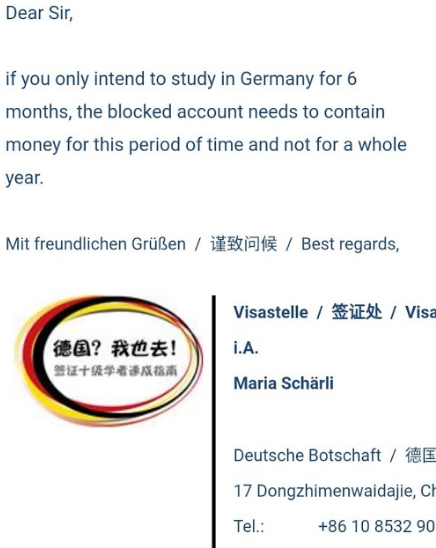
\includegraphics[height=.5\textheight]{email-from-Visa}
  \caption{德国使馆回信}
  \label{fig:email}
\end{figure}
\item[行程] 地铁一号线大望路站,刷卡(码)出站后,顺着 \textbf{\color{blue}A (东北)口}出站方向,前行约十米,沿着\textbf{\color{blue}“华贸中心”通道}前行。进入“华贸中心”(B1,负一层)后,按指示路牌 \textbf{\color{blue}“华贸写字楼”} 方向前行至一上行扶梯处。出扶梯左手入口即有``Deutsche Bank'' 标志。有服务人员在柜台等候。按指示在机器上选 27 层德意志银行,得到二维码。刷码进入写字中心。乘梯至 27 层,左手即为德意志银行。
\item[表格]
\begin{itemize}
  \item 请务必下载 \href{https://china.db.com/china/docs/1.opening\_a\_bank\_account\_for\_foreign\_students\_over18years.pdf}{\textbf{\color{blue}官方最新版表格}}. 填写完整后打印 ``Guidance notes'' 后的所有页(文档当前版本:
  007 91995 28 DBEN 164 WWW ERO BV VJ \textbf{\color{blue}181024} 的\textbf{\color{blue}第 9 -- 19 页}),包括 ``Schufa'' 1 页, ``Entgeltinformation'' 3 页和 ``Depositor Information Sheet'' 1 页。 
  \item 请确保自动生成了 ``\textbf{\color{blue}First name/s}'', ``\textbf{\color{blue}Surname}'' 两栏
  \item 身份证、护照页复印件\textbf{避免过黑}。在空白处写上个人 “姓名” + “拼音”(此前已经有人建议姓名全部大写。我全部大写了)
  \item 按照工作人员的意思,邮寄可能比自取\textbf{\color{blue}晚“一到两天”}。我选了邮寄。邮寄方式应该为 EMS.
  \item 银行张贴的开户示例与官网示例稍有不同---主要是“城市”全部写成“\textbf{\color{blue}省份+城市}”(或城市+省份。可由逗号或空格分隔。下同)。我拍了前两张,将发群里。
  \begin{itemize}
    \item ``Place of birth'' 省份 + 城市
    \item ``Regestered address'' 中 ``Town/City'' 省份 + 城市。我填了 ``BeijingShijingshan''. 没有空格,因为格数不够。
    \item ``My relationship with this person is as follows (e.g. father/son)'' 我填写了 ``Mother\textbf{\color{blue}/Son}''. 注意,后面的 ``/Son(/Daughter)'' \textbf{\color{blue}不可省}。
  \end{itemize}
\item JHX: 材料不要订起来
\item 据说华贸大厦马路对面有家打印店,可搜索到。打印费较贵, 0.5 元/张(ZZY:“那边打印店 2 元一张)。但我高德地图搜不到。仅需打印修改过的页面。{\color{blue}无需打印自己保留的那一份}。我是托旁边人一起打印的,打印店具体位置等不清楚。而且请注意{\color{blue}打印不清晰的,应要求重新打印}。我有几页打印太不清晰。幸好那几页所有人都相同,台湾的一位朋友把他剩余的那几页给了我。
\item 由于去中国银行、工商银行(均在华贸中心一楼。工商银行需转角出门再进。可询问服务台)\textbf{均需\color{blue}当前银行卡},暂不接受现金汇款;而我没有这两个银行的卡,于是我回到玉泉路建行汇出开户手续费。%据 ZJR 表示,德意志银行\textbf{\color{blue}不会通知}是否收到该笔汇款。我托ZZY明天问问德意志银行。
\\
% 这件事情最好有个彻底的处理方式。比如,要求银行受到汇款后发出通知。
ZZY:“关于汇款问题,假如你没汇款是会有电话通知。没问题就不会联系。”
\item 银行业务人员要求拍照保存自己填写的快递单。利用快递单,可以查看相应材料的运送进程。
\item 银行仅两个柜台。我当天仅一位业务人员。
\item 我全程感觉到的都是{\color{blue}和善}。业务人员也很耐心。本来办公时间只到 11:30, 但她允许我们最迟 12:00 递交材料。
\end{itemize}
\item[转账] 我利用建行网银向上述指定银行转账 8900 欧元。周一转出,当周五受到德银的“个人帐号通知函”(名称由申请开户时拿到的“个人编号通知单”推知)邮件。虽然过程中有以下小问题(及处理方式),但从结果来看,没有受到影响。
\begin{itemize}
  \item 建行网银转账时,输入对方账户名时,不能包含 ``Bank''. 我改为 "BK".
  \item 按开户表上填写的 8900 欧元,实际转出 8900 欧元。“个人帐号通知函”上显示,实际到帐 8870 欧元(应该是中转过程中扣除了 30 欧元)。
\end{itemize} 
\item[解冻] ( ZJR )回国前可以用\textbf{机票和学校的注销证明}去德意志银行解冻。
\end{description}

\chapter{1 月 17 日递签资料图表}\label{ap:visa-figures}
\begin{table}[htbp]
  \caption{递签简表}
  \centering
  \begin{tabular}{r|l}
    \toprule
    地点 & 亮马桥外交大楼 {\color{blue} D1 座 1302}【而非邮件里说的 E 座】 \\ \midrule
    流程 & 8:00 -- 9:00 取号、填写 EMS 邮寄单、整理比对递签材料 \\
    & 9:00 -- 12:00 逐一递签(我们这次时间延长到 12:30 左右。会保证每人至少一次递签机会) \\
    \bottomrule
  \end{tabular}
\end{table}
% 1.地点:亮马桥外交大楼 DI 座 1302【而非邮件里说的 E 座】 

% 2.虽然预约的时间是8:00-9:00,但其实九点才开始受理。但还是建议早点去,因为可以早点上去取号,取了号再下楼办EMS的邮寄单。这样可以防止取到的号比较靠后。 

% 3.等待的地方是一间小屋子,墙上有申请表的填写模板和递交材料的顺序,可以对照看自己的填写和材料的顺序。 

% 4.【等待的小屋子不许玩手机,不许用电脑,不许用电子设备。建议自备其他休闲娱乐方式】 

\section{材料顺序及 APS 模板}
\begin{figure}[htbp]
  \centering
  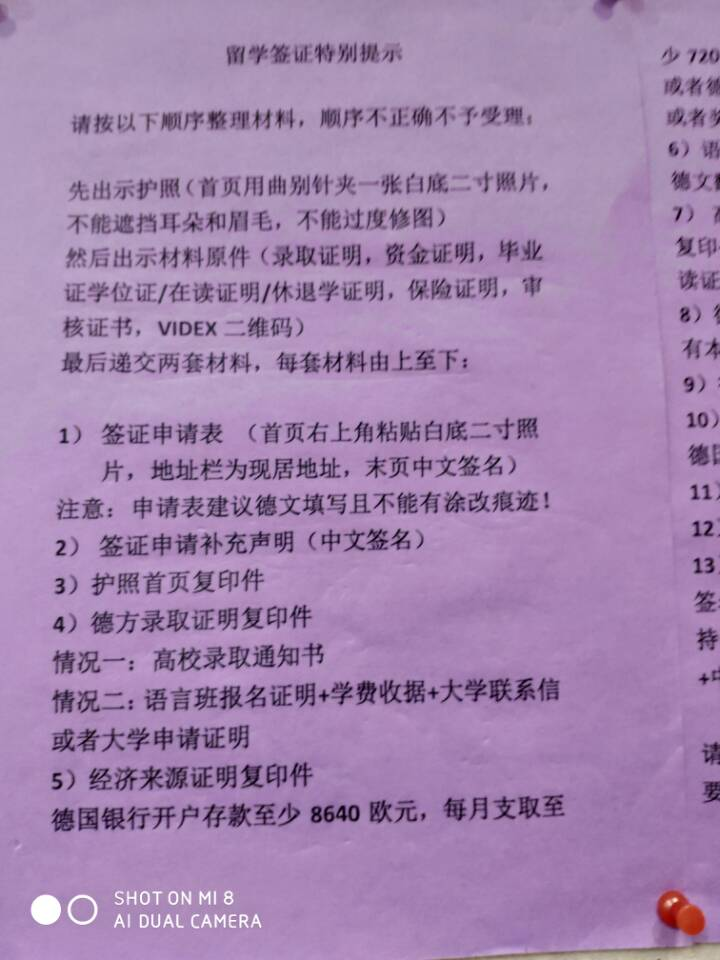
\includegraphics[width=\textwidth]{order-1}
  \caption{材料顺序要求第 1 页。摄于 2019 年 1 月 17 日}
  \label{fig:order-1}
\end{figure}
\begin{figure}[htbp]
  \centering
  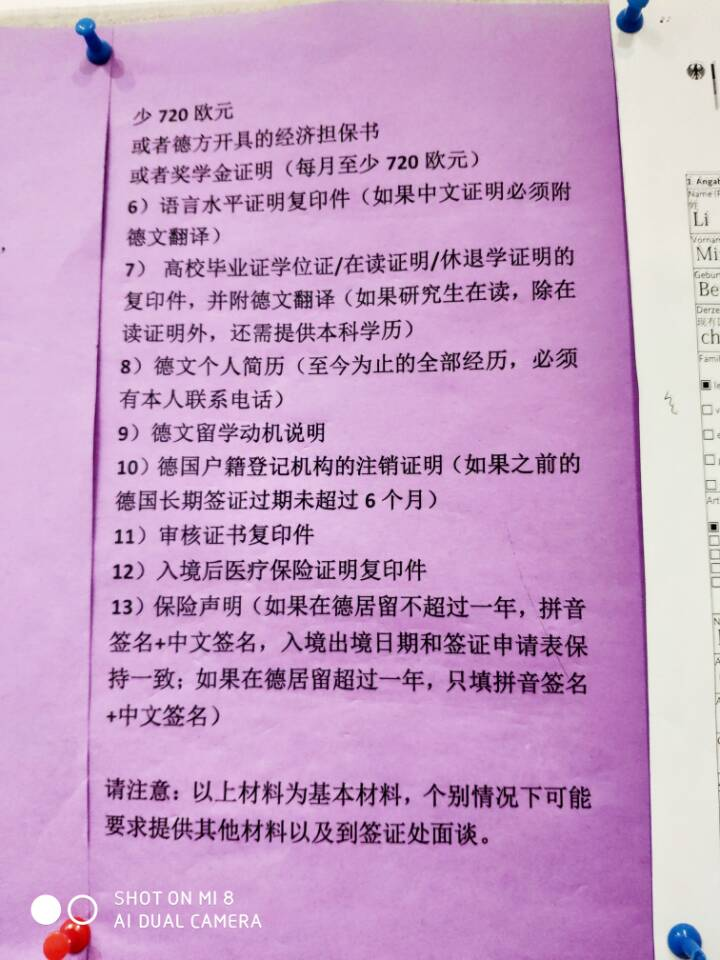
\includegraphics[width=\textwidth]{order-2}
  \caption{材料顺序要求第 2 页。摄于 2019 年 1 月 17 日}
  \label{fig:order-2}
\end{figure}
\begin{figure}[htbp]
  \centering
  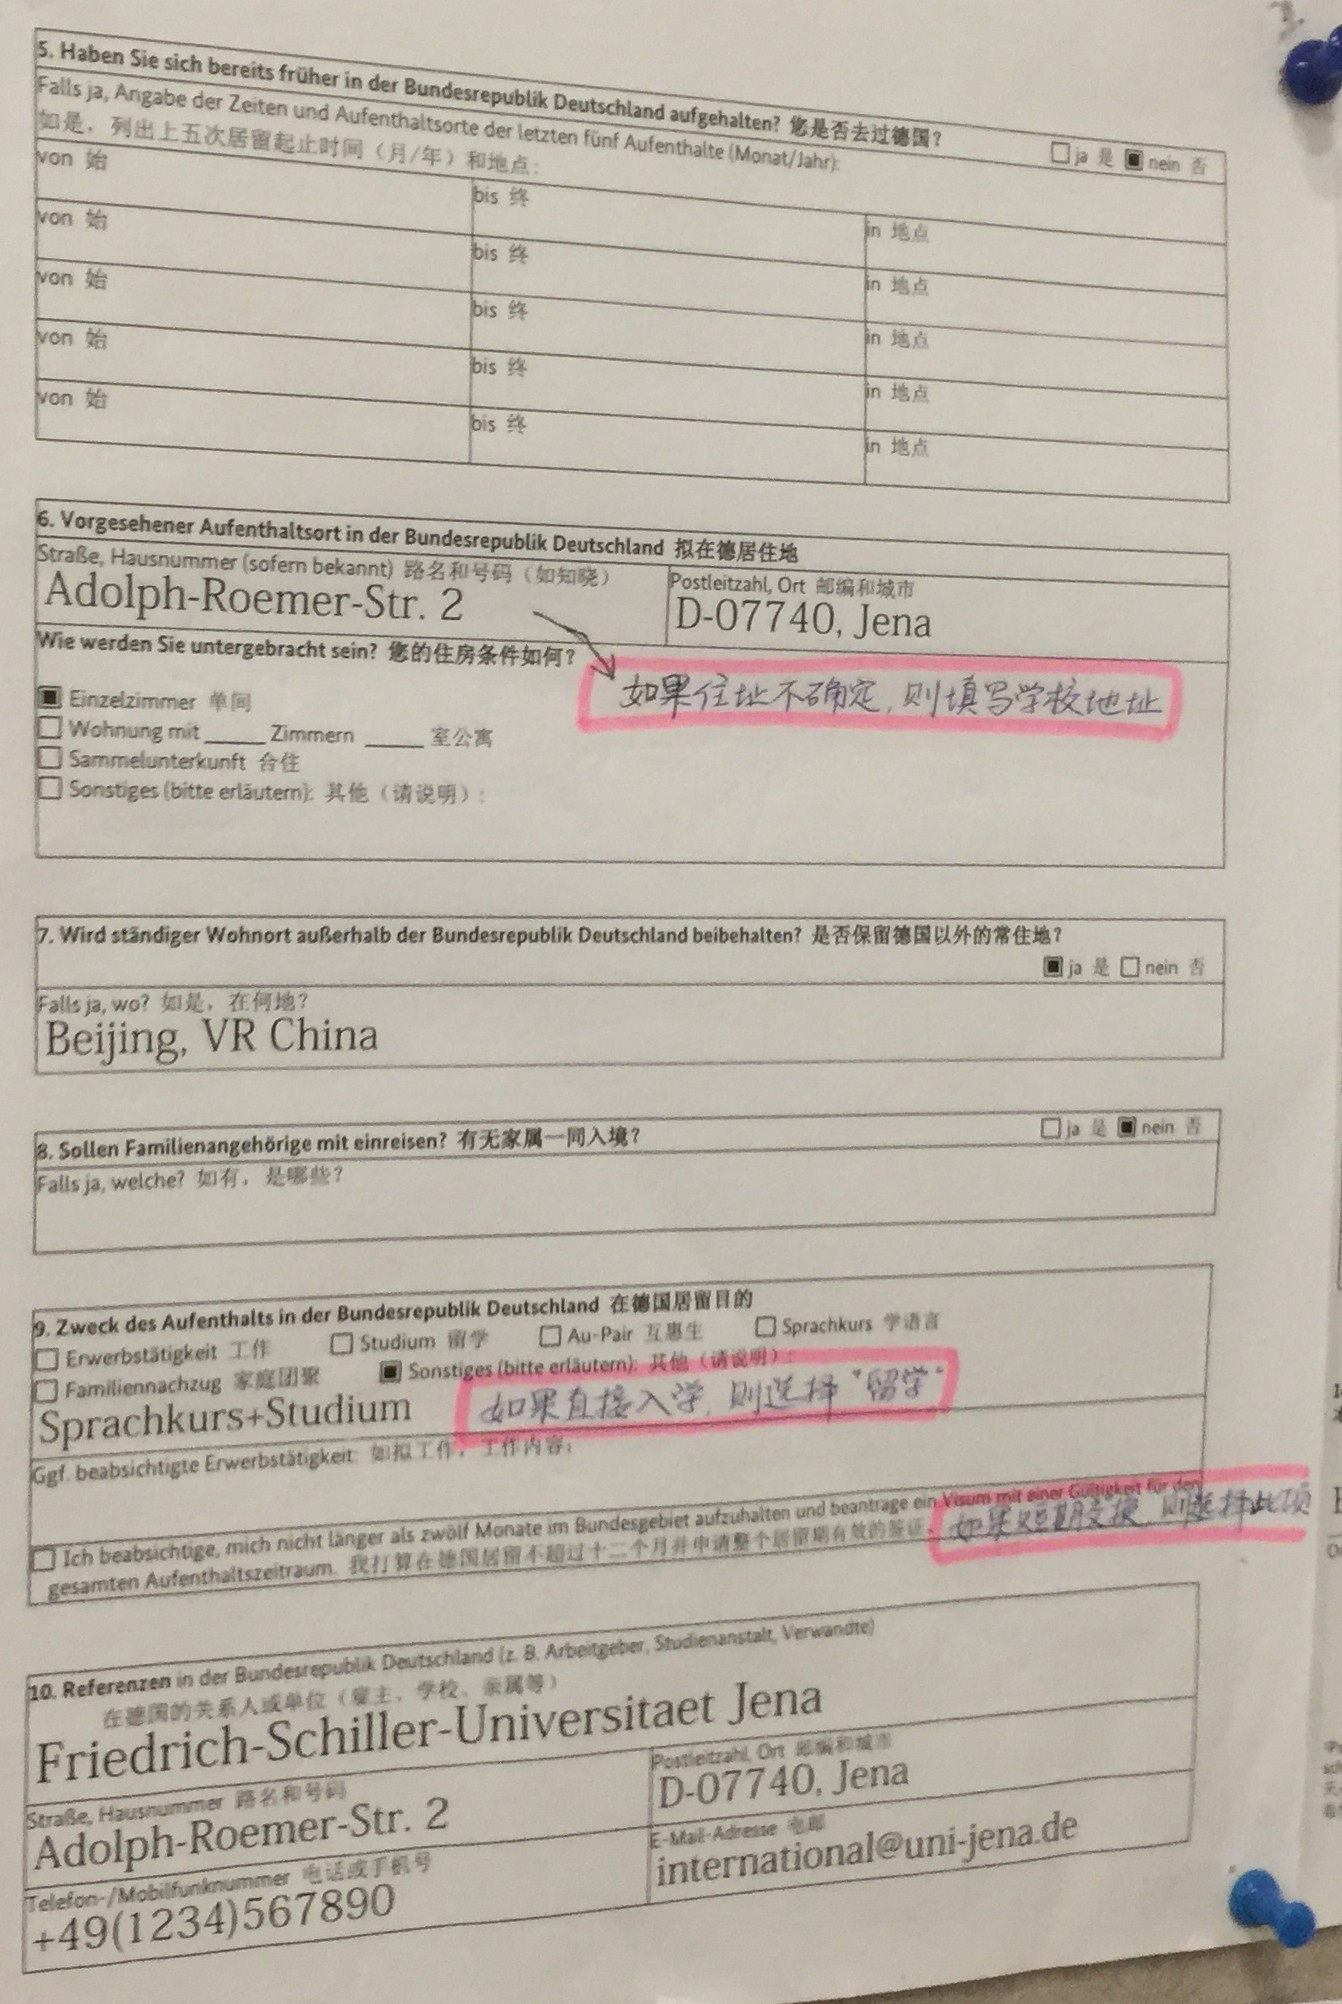
\includegraphics[width=\textwidth]{APS-forms}
  \caption{APS 申请表填写模板。摄于 2019 年 1 月 17 日}
  \label{fig:APS-forms}
\end{figure}

\section{路线图}
\begin{figure}[htbp]
  \centering
  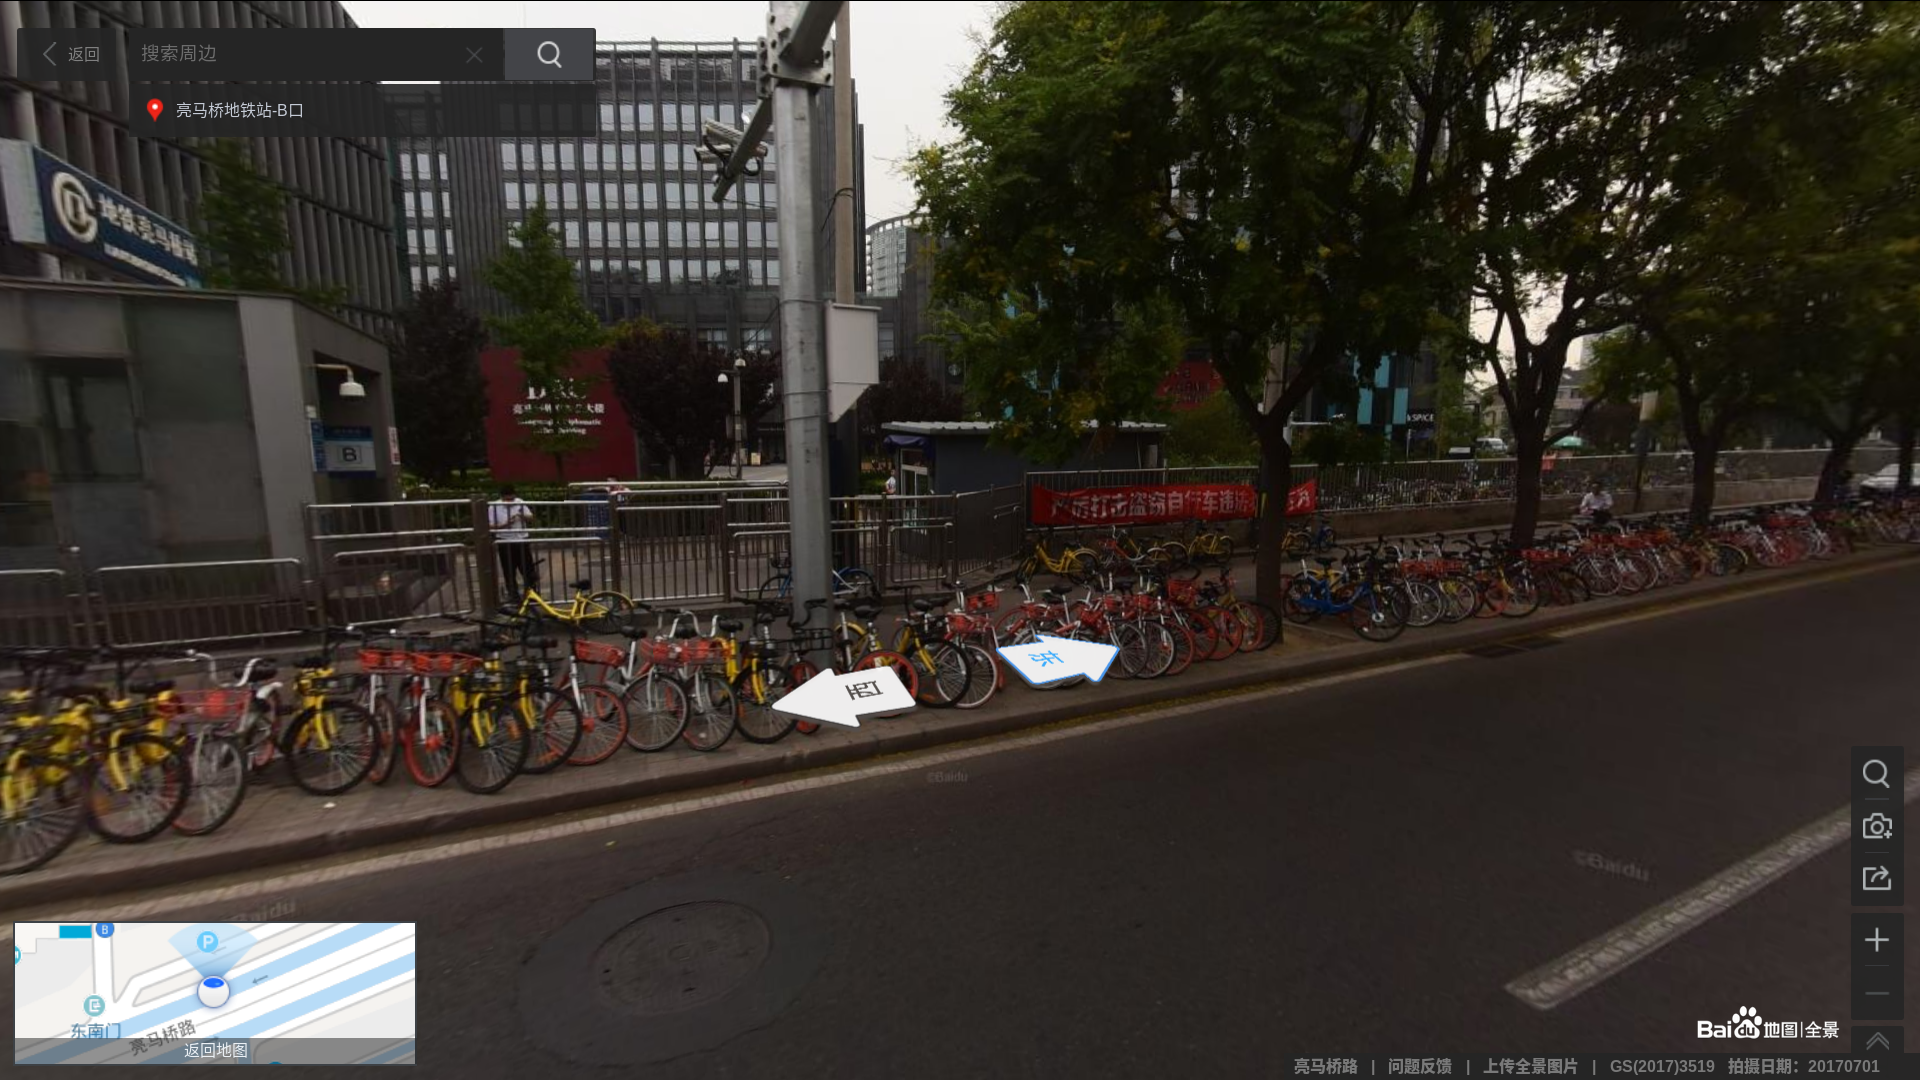
\includegraphics[width=\linewidth]{metro-B}
  \caption[亮马桥地铁 B 口]{亮马桥地铁 B 口。截图来自 \href{https://map.baidu.com/\#panoid=09002200121707010630058282I\&panotype=street\&heading=0.64\&pitch=-4.92\&l=19\&tn=B_NORMAL_MAP\&sc=0\&newmap=1\&shareurl=1\&pid=09002200121707010630058282I}{百度全景}。}
  \label{fig:real}
\end{figure}
\begin{figure}
  \centering
  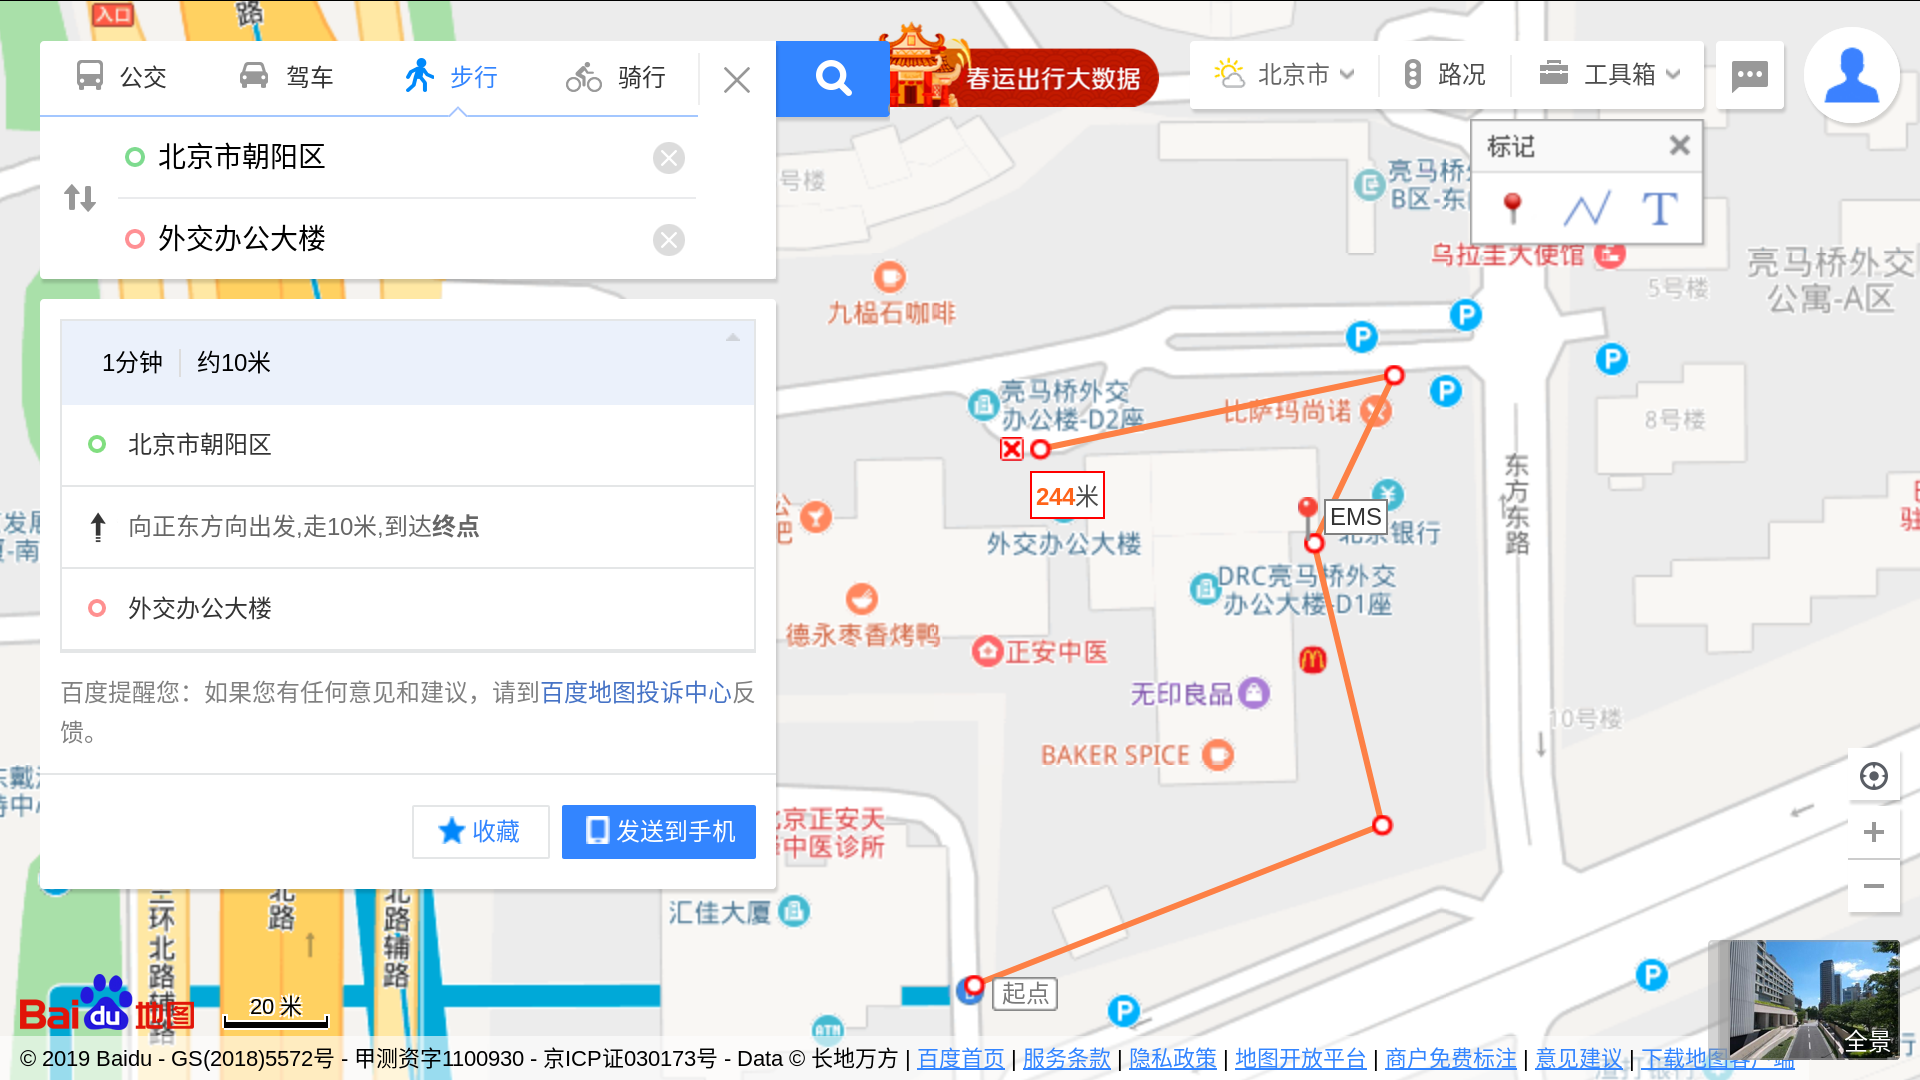
\includegraphics[width=\linewidth]{route-to-D1}
  \caption[地铁 B 口前往 D1 座路线]{地铁 B 口前往 D1 座路线。路经 EMS. 截图来自\href{https://map.baidu.com/}{百度地图}。}
  \label{fig:route}
\end{figure}
\begin{figure}
  \centering
  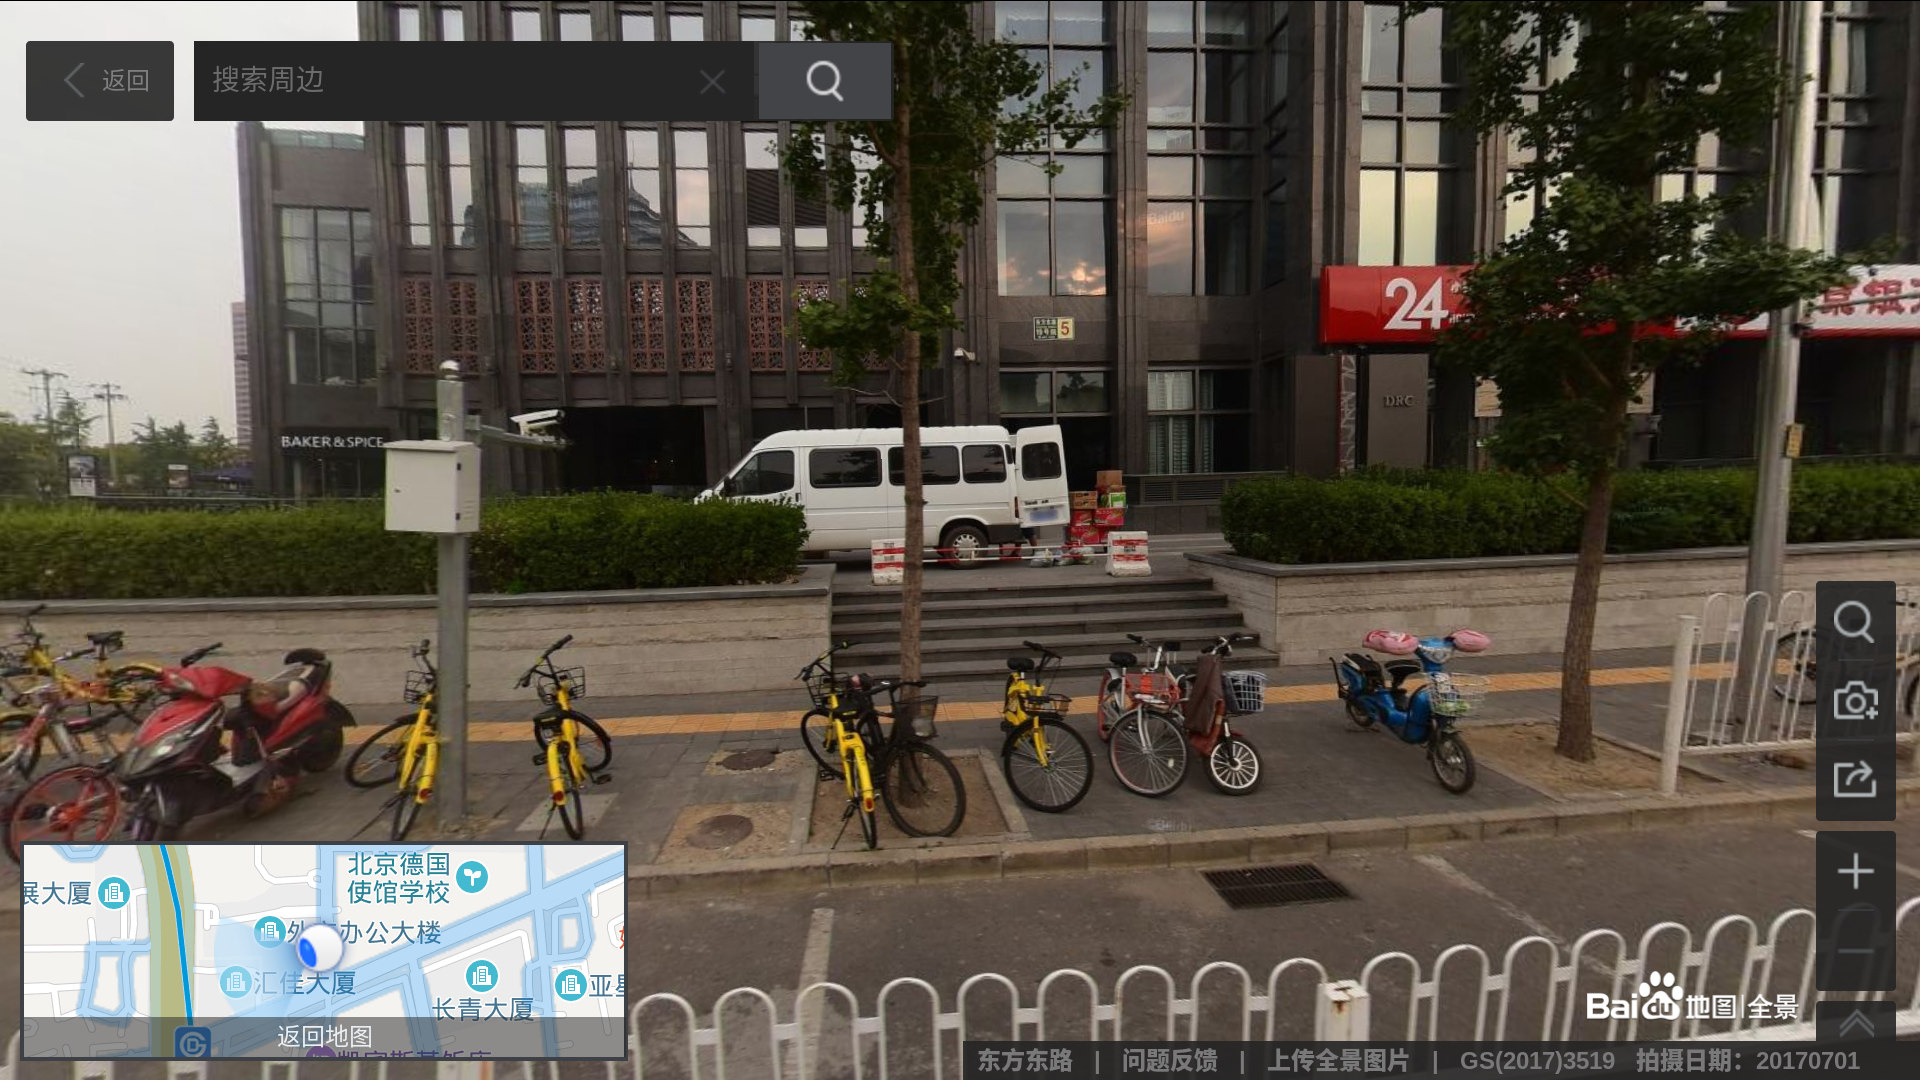
\includegraphics[width=\linewidth]{EMS}
  \caption[EMS 办理处]{EMS 办理处。应该是在图中汽车的后面,并从车的左侧进入通道。截图来自\href{https://map.baidu.com/\#panoid=09002200121707010635276742I\&panotype=street\&heading=274.99\&pitch=-2.29\&l=12\&tn=B_NORMAL_MAP\&sc=0\&newmap=1\&shareurl=1\&pid=09002200121707010635276742I}{百度地图}。我当时忘了拍照。抱歉。}
  \label{fig:EMS}
\end{figure}

% 1.护照(首页用曲别针夹一张白底二寸照片,不能遮挡耳朵和眉毛, 不能过度修图) 

% 2.材料原件(EMS邮寄单、VIDEX二维码录取证明、资金证明、在读证明、保险证明、审核证书、联系人说明) 

% 【备注:保险证明最好把 AOK 邮件里的两个附件都打印了。一定记得带上联系人说明】 

% 三、然后递交两套材料,每套材料由上至下按如下顺序放置【顺序不对不予受理】: 

% 1.签证申请表 (首页右上角粘贴白底二寸照片, 地址栏为现居地址, 末页中文签名) 

% 注意:申请表建议德文填写且不能有涂改痕迹! 

% 【签证申请表填写细节与学长的模板不太一致!!!】 

% 2.签证申请补充声明(中文签名) 

% 3.护照首页复印件 

% 4.德方录取证明复印件:高校录取通知书 

% 5.经济来源证明复印件 

% 6.语言水平证明复印件(如果中文证明必须附德文翻译) 

% 7.在读证明复印件,并附德文翻译 

% 8.德文个人简历(至今为止的全部经历,必须有本人联系电话) 

% 9.德文留学动机说明 

% 10.审核证书复印件 

% 11.医疗保险证明复印件 

% 12.保险声明(如果在德居留不超过一年,拼音签名+中文签名,入境出境日期和签证申请表保持一致) 

% 四、材料审核没有问题后录指纹 

 

% 血泪教训: 
\end{appendices}
\end{document}